% !TEX root = ../thesis.tex
The first problem examined is a so called Poiseuille flow, which is one of the simplest nontrivial cases in incompressible fluid dynamics.
It's a stationary flow in a pipe, driven by a pressure gradient through it.
Due to the wall friction, this leads to a parabolic flow, which we will use as inflow condition.

\begin{figure}[h!]
  \centering
  % !TEX root = ../../thesis.tex

\begin{tikzpicture}
\fill[pattern=north east lines] (0,0) rectangle (10,-0.2);
\fill[pattern=north east lines] (0,3) rectangle (10,3.2);
\draw (0,0) .. controls (3,1) and (3,2) .. (0,3);

\draw[gray, dashed]  (5,0) -- (5,3);

\draw (0,0) -- (10,0);
\draw (0,3) -- (10,3);
\draw (0,0) -- (0,3);

\draw[->] (0,1.5) -- (2.25,1.5);
\draw[->] (0,1) -- (2,1);
\draw[->] (0,2) -- (2,2);
\draw[->] (0,2.5) -- (1.22,2.5);
\draw[->] (0,0.5) -- (1.22,0.5);


\node (u) at (1.1,1.7) {$\vec{u}$};


\draw[->] (-0.5,-0.7) -- (-0.5,4);
\draw[->] (-0.5,-0.7) -- (10.5,-0.7);

\node (y) at (-0.5,4.2) {$y$};
\node (x) at (10.7,-0.7) {$x$};

\draw[-] (-0.55,1.5) -- (-0.45,1.5);
\draw[-] (0,-0.65) -- (0,-0.75);
\draw[-] (5,-0.65) -- (5,-0.75);
\draw[-] (10,-0.65) -- (10,-0.75);

\node (nully) at (0,-0.95) {$0$};
\node (L) at (10,-0.95) {$L$};
\node (Lh) at (5,-1.) {$L/2$};
\node (nullx) at (-0.65,1.5) {$0$};
\end{tikzpicture}

  \caption{Setup for Poiseuille flow. Velocity is measured at $\frac{L}{2}$.}
\label{fig: poiseuille}
\end{figure}

Figure~\ref{fig: poiseuille} shows a schematic of the setup.
The test examines the influence of the length of the channel\footnote{To be exact, the following lengths are simulated:\par
 $100,\ 95,\ 90,\ 85,\ 80,\ 75,\ 70,\ 65,\ 60,\ 55,\ 50,\ 45,\ 40,\ 35,\ 30,\ 25,\ 20,\ 15,\ 11,\ 9,\ 7,\ 5,\ 3$
} on the velocity distribution in the middle column.
The height is always chosen to be $20$ cells.

As the \gls{lbm} is a mildly compressible scheme, the comparison with the incompressible, analytic result would not be very expressive.
Indeed, the velocities computed with either method are decreasing in comparison with the analytic result when choosing longer channels.
Instead, the difference between the velocities computed with Cumulants and \gls{srt} in the middle of the channel length is taken and summed up over the channel height.

\begin{figure}
  \centering
  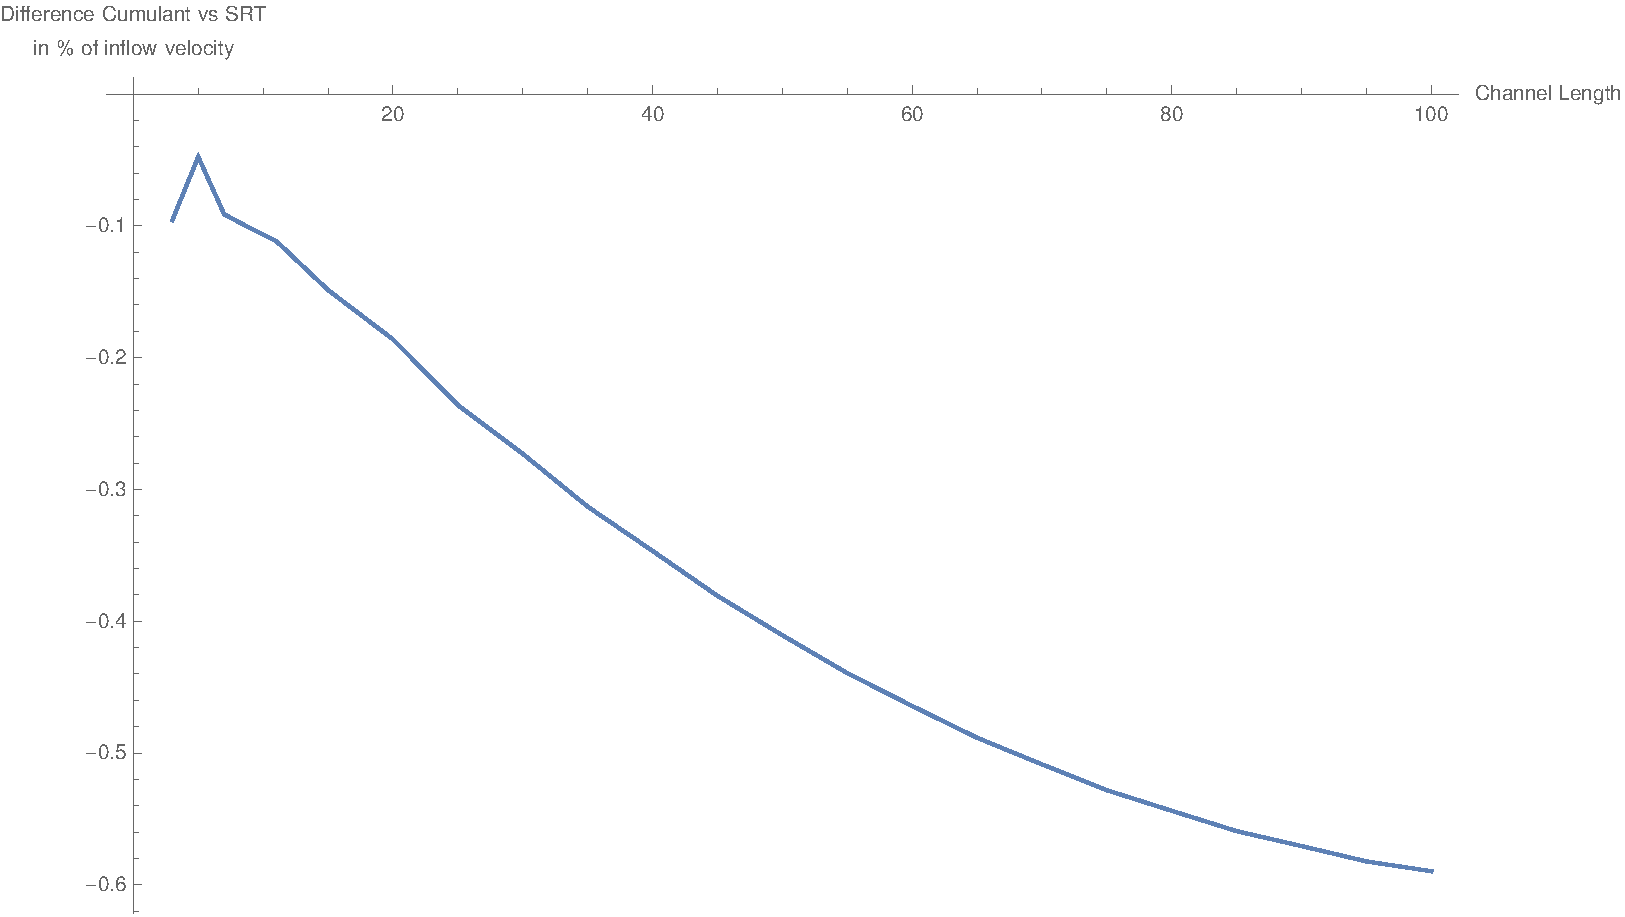
\includegraphics[width=0.8\linewidth]{../figures/poiseuille.pdf} % chktex 11
  \caption{Difference between Cumulants and SRT in percent of the initial inflow velocity in a Poiseuille Flow plotted agains the channel length}
\label{fig: poiseuille result}
\end{figure}

The result can be seen in Figure~\eqref{fig: poiseuille result}.
Two things are remarkable here.
First of all, the difference is below one percent of the inflow velocity which is a first sign, that the Cumulant is not completely off the track.

Secondly, we can look at the nature of the difference.
Here, we see that the velocity in the case of Cumulants was generally a bit more slowed down than \gls{srt}, which indicates, that the cumulant method treats the fluid a bit more compressible.

We can conclude, that Cumulants give meaningful results in this case.
To spot the different behavior of the two methods, we move on to some more challenging tasks.
